\documentclass[compress]{beamer}
%pour virer les effets:
%\documentclass[handout]{beamer}

\usepackage[utf8]{inputenc}
\usepackage[T1]{fontenc}
\usepackage[francais]{babel}
\usepackage{graphicx,tikz}
\usepackage{xcolor}
\usepackage{multicol}
\usepackage{template}

\usetikzlibrary{automata}

\useoutertheme[subsection=false]{miniframes}

%%%%%%%%%%%%%%%%%%%%%%%%%%%%%%%%%%%%%%%%%%%%%%%%%%%%%%%%%%%%%%%%%%%%%%%%

\errorcontextlines=5

\newcommand{\deroulementJeu}[4][12em]{%
  \begin{columns}
    \begin{column}[l]{.20\linewidth}
      \includegraphics[width=1.\linewidth]{images/#2}
    \end{column}

    \begin{column}[c]{.60\linewidth}
      \begin{center}
        \noindent
        \smash{\includegraphics[width=#1]{images/#3}}
        \par\vfill
      \end{center}
    \end{column}
    \begin{column}[r]{.20\linewidth}
      \includegraphics[width=1.\linewidth]{images/#4}
    \end{column}
  \end{columns}
}

%%%%%%%%%%%%%%%%%%%%%%%%%%%%%%%%%%%%%%%%%%%%%%%%%%%%%%%%%%%%%%%%%%%%%%%%

\title{Atelier de robotique}
\subtitle{Puissance 4}
\author[Institut de Mathématique]{%
  Sabrina \textsc{Dassonville}
  \and Vinciane \textsc{De Waele}
  \and Florine \textsc{Frist}
  \and David \textsc{Sbabo}
  \and Christophe~\textsc{Troestler}}
\date{Printemps des Sciences, mars 2010}
\institute{UMONS}



\begin{document}

\frame {
	\maketitle
}

\section*{Introduction}
\frame {
	\frametitle{Introduction}
	\textbf{Objectif :} Construire un robot qui joue à puissance 4.\\
	\vspace{.8em}
	\textbf{Deux aspects :}\\
	\begin{itemize}
		\item construction en Lego
		\begin{itemize}
			\item mettre les pièces dans la grille
			\item détecter la pièce ajoutée par l'utilisateur
		\end{itemize}
		\item programmation
		\begin{itemize}
			\item déplacements du robot 
			\item intelligence artificielle
		\end{itemize}
	\end{itemize}
}

\frame {
	\frametitle{Plan}
	\tableofcontents
}

\section{Construction du robot}
\frame {
	\frametitle{Construction du robot}
	\begin{Large}
		Au début, il y avait ...
 	\end{Large}
 	\pause
 	\begin{center}
		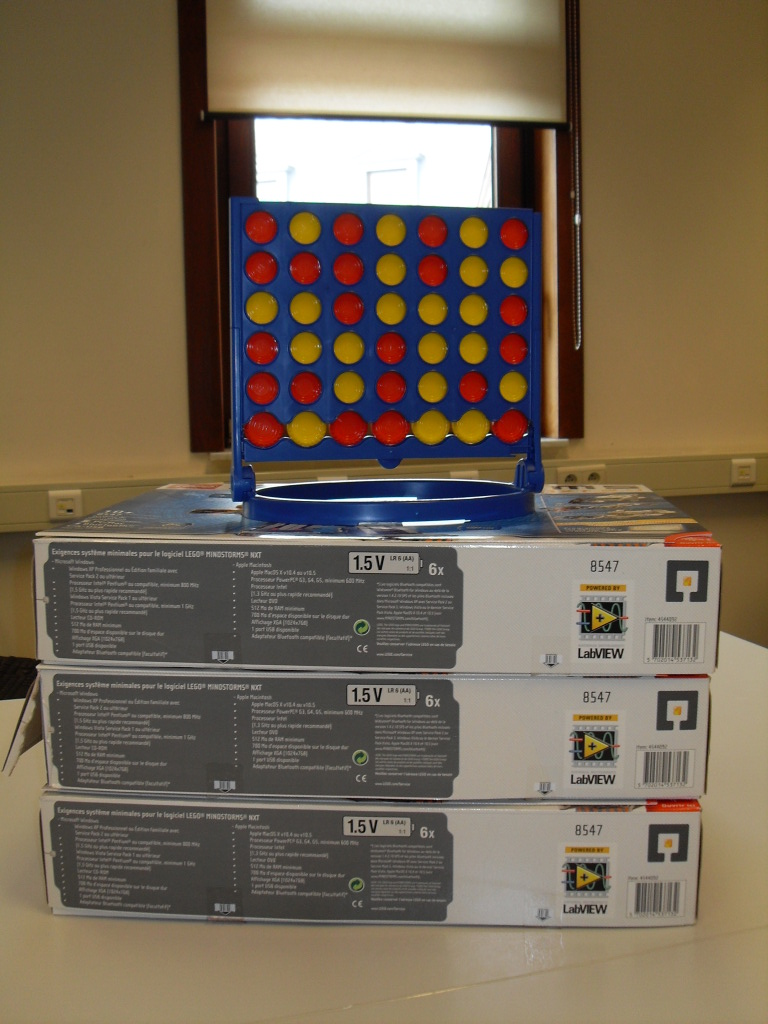
\includegraphics[width=0.43\linewidth]{images/boite.jpg}
 	\end{center}
}

\frame {
	\frametitle{Construction du robot}
	\begin{center}
		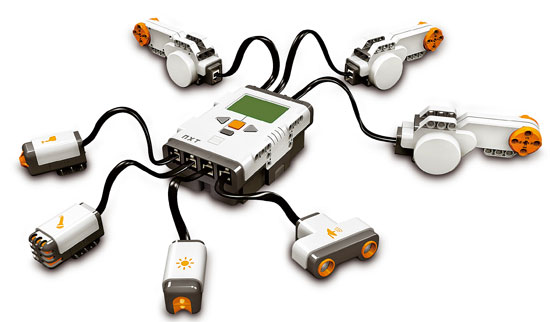
\includegraphics[width=0.7\linewidth]{images/mindstorm1.jpg}
 	\end{center}
}

\frame {
	\frametitle{Construction du robot}
 	\begin{Large}
		Mais aussi et surtout ...
 	\end{Large}
 	\pause
 	\begin{center}
		
\includegraphics[width=0.25\linewidth]{images/reflexion.png}
	\end{center}
}

\frame {
	\frametitle{Construction du robot}
	\begin{large}
		En effet, cela nous a demandé beaucoup d'imagination :
	\end{large}
	\begin{columns}
		\begin{column}{.6\linewidth}
			\begin{center}
				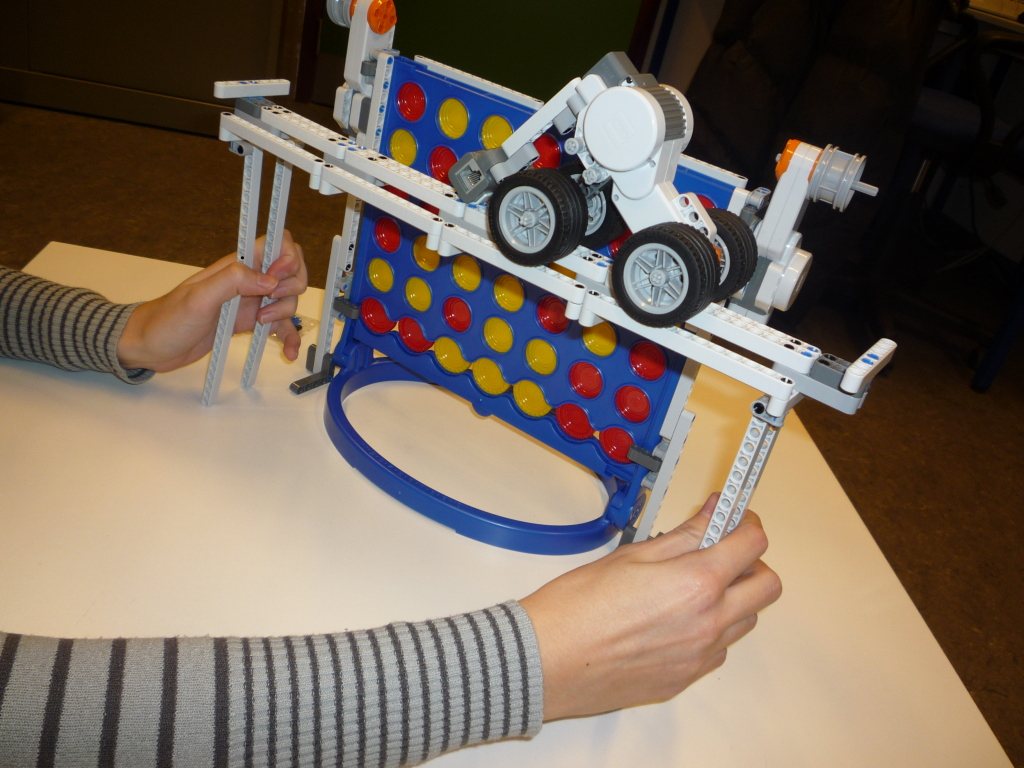
\includegraphics[width=1\linewidth]{images/4X4.jpg}
			\end{center}
		\end{column}
		\begin{column}{.38\linewidth}
			\textbf{Inconvénients :}
			\begin{itemize}
				\item instable
				\item trop lourd
				\item précision des moteurs
			\end{itemize}
		\end{column}
	\end{columns}
}

\frame {
	\frametitle{Construction du robot}
	\begin{large}
		Première amélioration :
	\end{large}
	\begin{columns}
		\begin{column}{.4\linewidth}
			\begin{center}
				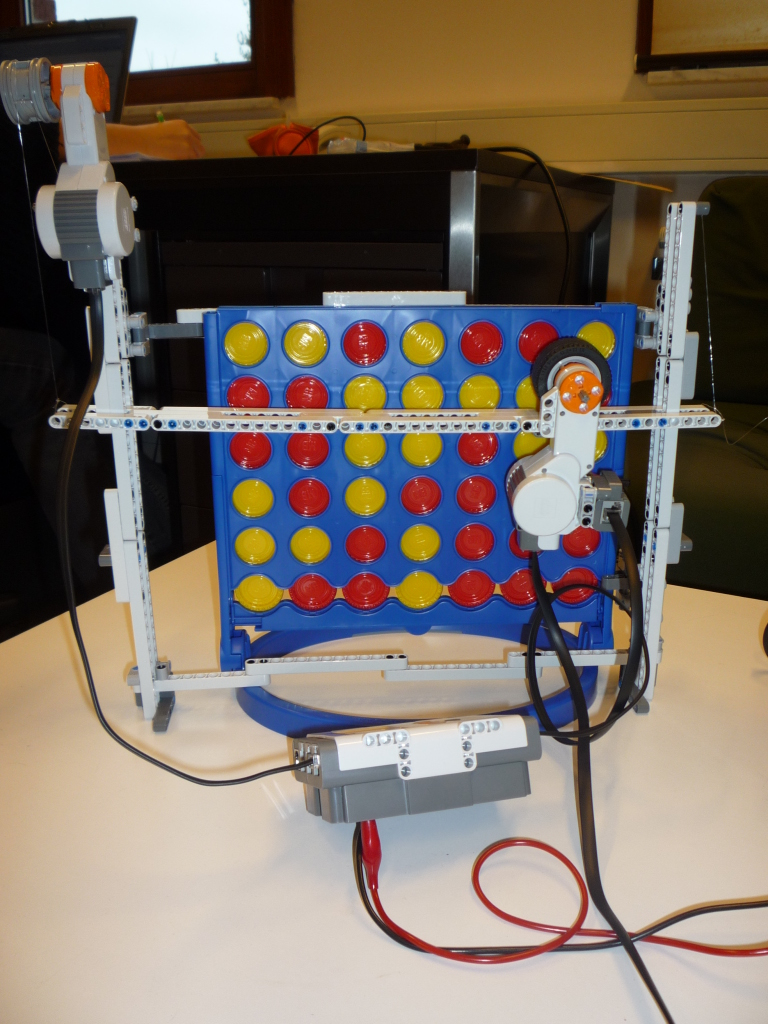
\includegraphics[width=1\linewidth]{images/capteurV2.jpg}
			\end{center}
		\end{column}
		\begin{column}{.6\linewidth}
			\textbf{Avantages :}
			\begin{itemize}
				\item stabilité
				\item plus léger
			\end{itemize}
			\textbf{Inconvénients :}
			\begin{itemize}
				\item besoin de placer le capteur en bas pour scanner la ligne du bas
				\item besoin de monter les guides plus haut
				\item problème de précision du capteur à cause de la rigidité des cables
			\end{itemize}
		\end{column}
	\end{columns}
}

\frame {
	\frametitle{Construction du robot}
	\begin{large}
		Avec la pince :
	\end{large}
	\begin{center}
		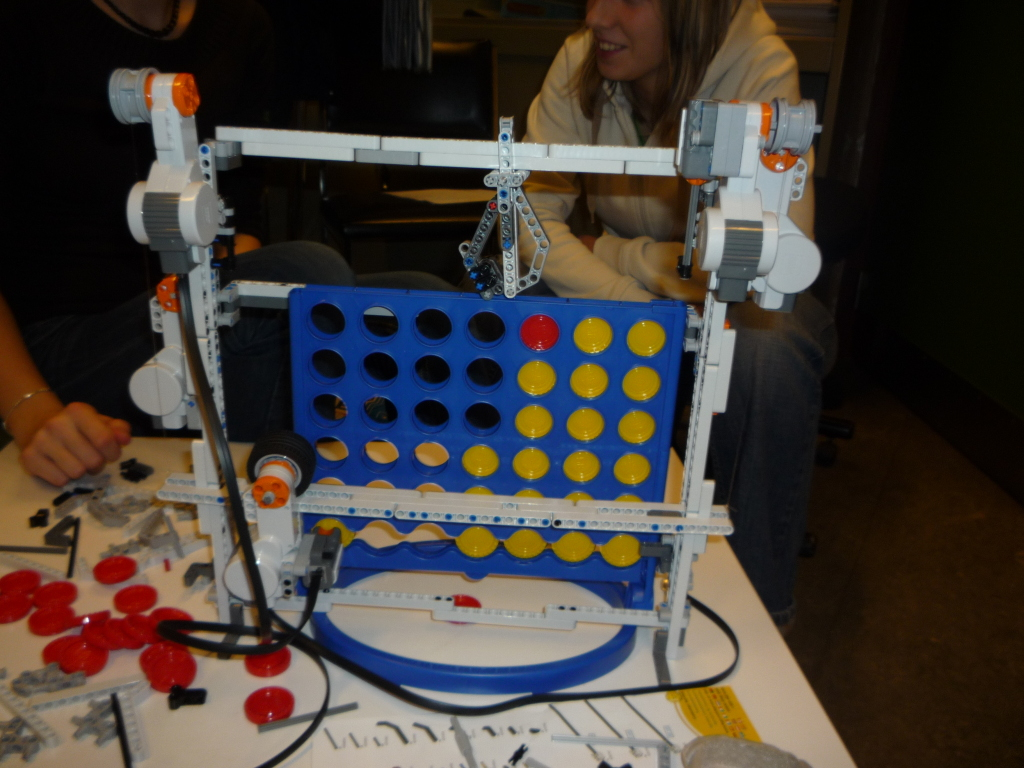
\includegraphics[width=0.78\linewidth]{images/pince.jpg}
	\end{center}
}

\frame {
	\frametitle{Construction du robot}
	\begin{center}
		
\includegraphics[width=0.55\linewidth]{images/cassetete.jpg}
	\end{center}
}

\frame {
	\frametitle{Construction du robot}
	\begin{Large}
		Cependant, nous y sommes arrivés!\\
		\pause
		Et en voici le résultat :
	\end{Large}
	
	\begin{columns}
		\begin{column}{.41\linewidth}
			\begin{center}
				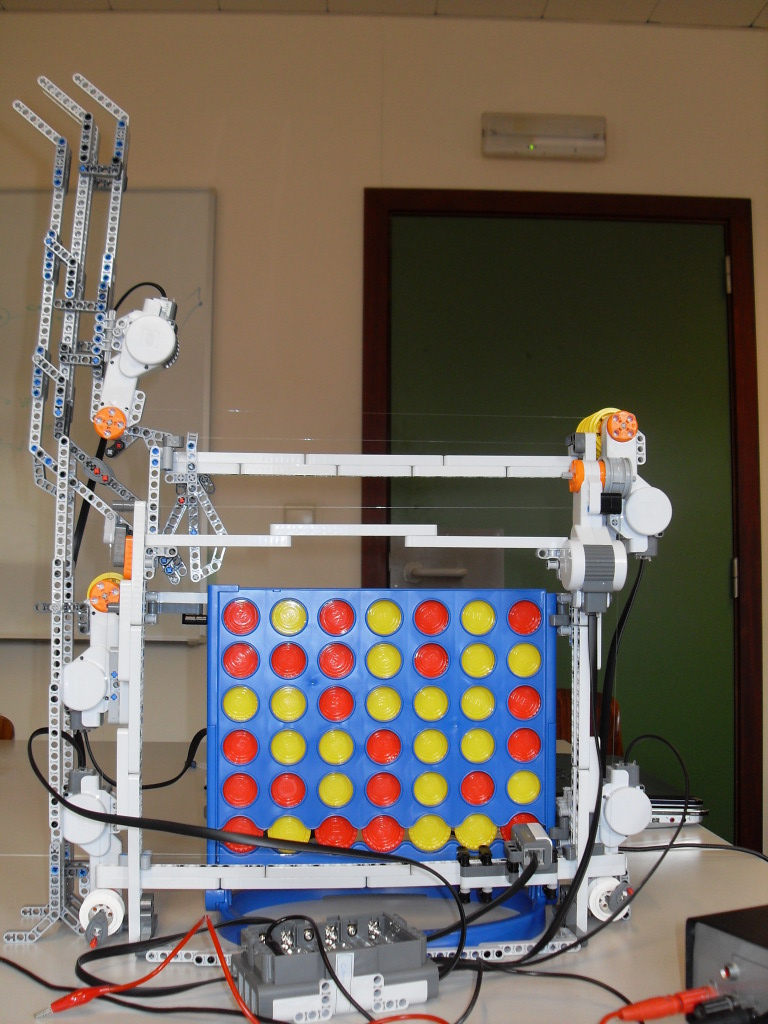
\includegraphics[width=1\linewidth]{images/final.jpg}
			\end{center}
		\end{column}
		\begin{column}{.5\linewidth}
			\textbf{Avantages :}
			\begin{itemize}
				\item stabilité
				\item légèreté
				\item simplicité
			\end{itemize}
			\textbf{Inconvénient :}
			\begin{itemize}
				\item tension dans les fils
			\end{itemize}
		\end{column}
	\end{columns}
}

\section{Règles du jeu}
\frame {
	\frametitle{Règles du jeu}
		\begin{itemize}
		\item Chaque joueur dispose de 21 pions.
		\item Les deux joueurs placent à tour de rôle un pion dans la
			colonne de leur choix.
		\item Le but est d'aligner au moins 4 pions horizontalement,
			verticalement ou diagonalement.
		\item Si la grille est complète et qu'aucun des deux joueurs
		n'a réussi à aligner au moins 4 pions, la partie est déclarée
		nulle.
	\end{itemize}
}

\frame {
	\frametitle{Défi}
	\begin{center}
		\begin{Huge}
			Défi !
		\end{Huge}
	\end{center}
}

\section{Idée de l'algorithme}
\frame{
	\frametitle{Stratégie}
	\begin{itemize}
		\item Il a été prouvé qu'il existe une stratégie gagnante pour le
		\textbf{1er joueur}.
		\pause
		\item Que signifient ces termes?
	\end{itemize}
	\pause
	\begin{block}{Stratégie gagnante}
		Une stratégie est dite gagnante pour un joueur J si, quelle
		que soit la façon dont joue l'autre joueur, le joueur J
		gagne en suivant cette stratégie.
	\end{block}
}

\subsection{Principe de base}
\begin{frame}
  \frametitle{Idée de l'algorithme}
 % \deroulementJeu[8em]{jeu_vide.png}{arbre.png}{jeu_vide.png}
    \begin{tikzpicture}[x=3em,y=2.3em,thick]
      \begin{scope}[text height=7pt]
        \node (top) [circle,draw] at (0,0) {};
        \node (l) [circle,draw] at (-2,-1.25) {};
        \onslide<2->{\node [circle,fill=red] at (l) {};}
        \node (c) [circle,draw] at (0,-1.25) {};
        \node (r) [circle,draw] at (2,-1.25) {};
        \draw[->] (top) -- (l) node[above,pos=0.5]{} ;
        \draw[->] (top) -- (c) node[left,pos=0.5] {};
        \draw[->] (top) -- (r) node[above,pos=0.5] {};
        \onslide<2->{%
          \node(ll) [circle,draw] at (-3.5,-2.5) {};
          \node(lc) [circle,draw] at (-2,-2.5) {};
          \onslide<3-6,12>{\node [circle,fill=yellow] at (lc) {};}
          \node(lr) [circle,draw] at (-0.5,-2.5) {};
          \onslide<7->{\node [circle,fill=yellow] at (lr) {};}
          \draw[->] (l) -- (ll) node[above,pos=0.5]{} ;
          \draw[->] (l) -- (lc) node[above left,pos=0.5] {};
          \draw[->] (l) -- (lr) node[above,pos=0.5] {};}
      \end{scope}
      \begin{scope}[text height=3pt]
        \onslide<3-6,12>{%
          \node (lcl) [circle,draw] at (-2.5,-4){};
          \onslide<4-6,12>{\node [circle,fill=red] at (lcl) {};}
          \node (lcc) [circle,draw] at (-2,-4) {};
          \node (lcr) [circle,draw] at (-1.5,-4) {};
          \draw[->] (lc) -- (lcl) node[above,pos=0.5]{} ;
          \draw[->] (lc) -- (lcc) node[above left,pos=0.5] {};
          \draw[->] (lc) -- (lcr) node[above,pos=0.5] {};
        }
        \onslide<4-6,12>{%
          \node (lcll) [circle,draw] at (-3,-5){};
          \node (lclc) [circle,draw] at (-2.5,-5) {};
          \onslide<5-6,12>{\node [circle,fill=yellow] at (lclc) {};}
          \node (lclr) [circle,draw] at (-2,-5) {};
          \draw[->] (lcl) -- (lcll) node[above,pos=0.5]{} ;
          \draw[->] (lcl) -- (lclc) node[above left,pos=0.5] {};
          \draw[->] (lcl) -- (lclr) node[above,pos=0.5] {};
        }
        \onslide<5-6,12>{%
          \node (lclcl) [circle,draw] at (-3,-6){};
          \node (lclcc) [circle,draw] at (-2.5,-6) {};
          \node (lclcr) [circle,draw] at (-2,-6) {};
          \draw[->] (lclc) -- (lclcl) node[above,pos=0.5]{} ;
          \draw[->] (lclc) -- (lclcc) node[above left,pos=0.5] {};
          \draw[->] (lclc) -- (lclcr) node[above,pos=0.5] {};
        }

        \onslide<6,12>{%
          \node [circle,fill=red] at (lclcl){%
            \rlap{\hss\smash{\raisebox{-0.3ex}{\onslide<12>{G}}}}};
        }

        \onslide<7->{%
          \node (lrl) [circle,draw] at (-1.,-4){};
          \node (lrc) [circle,draw] at (-0.5,-4) {};
          \onslide<8->{\node [circle,fill=red] at (lrc) {};}
          \node (lrr) [circle,draw] at (0,-4) {};
          \draw[->] (lr) -- (lrl);
          \draw[->] (lr) -- (lrc);
          \draw[->] (lr) -- (lrr);
        }

        \onslide<8->{%
          \node(lrcl) [circle,draw] at (-1,-5){};
          \node(lrcc) [circle,draw] at (-0.5,-5){};
          \node(lrcr) [circle,draw] at (0,-5){};
          \onslide<9->{\node [circle,fill=yellow] at (lrcr) {};}
          \draw[->] (lrc) -- (lrcl);
          \draw[->] (lrc) -- (lrcc);
          \draw[->] (lrc) -- (lrcr);
        }

        \onslide<9->{%
          \node(lrcrl) [circle,draw] at (-0.5,-6){};
          \node(lrcrc) [circle,draw] at (0,-6){};
          \onslide<10->{\node [circle,fill=red] at (lrcrc) {};}
          \node(lrcrr) [circle,draw] at (0.5,-6){};
          \draw[->] (lrcr) -- (lrcrl);
          \draw[->] (lrcr) -- (lrcrc);
          \draw[->] (lrcr) -- (lrcrr);
        }

        \onslide<10->{%
          \node(lrcrcl) [circle,draw] at (-0.5,-7){};
          \node(lrcrcc) [circle,draw] at (0,-7){};
          \node(lrcrcr) [circle,draw] at (0.5,-7){};
          \draw[->] (lrcrc) -- (lrcrcl);
          \draw[->] (lrcrc) -- (lrcrcc);
          \draw[->] (lrcrc) -- (lrcrcr);
        }

         \onslide<11->{%
          \node [circle,fill=yellow] at (lrcrcr){%
            \rlap{\hss\smash{\raisebox{-0.3ex}{\onslide<12>{P}}}}};
        }
      \end{scope}

    \end{tikzpicture}
    \hfill
    \only<1>{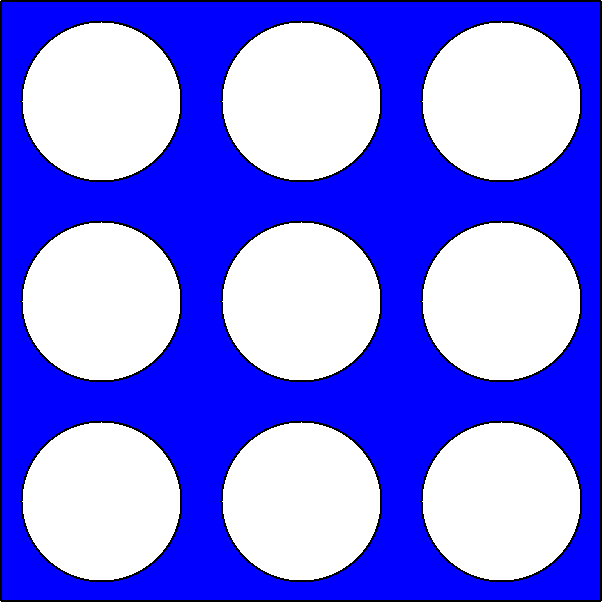
\includegraphics[width=0.25\linewidth]{images/jeu_vide.png}}%
    \only<2>{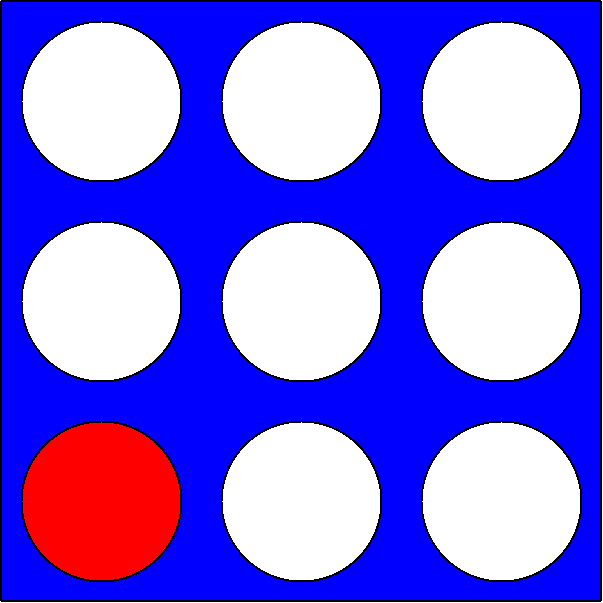
\includegraphics[width=0.25\linewidth]{images/1er.png}}%
    \only<3>{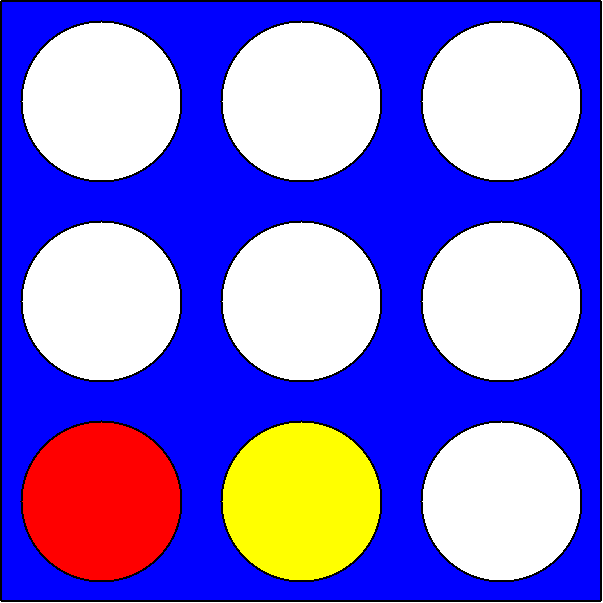
\includegraphics[width=0.25\linewidth]{images/2e.png}}%
    \only<4>{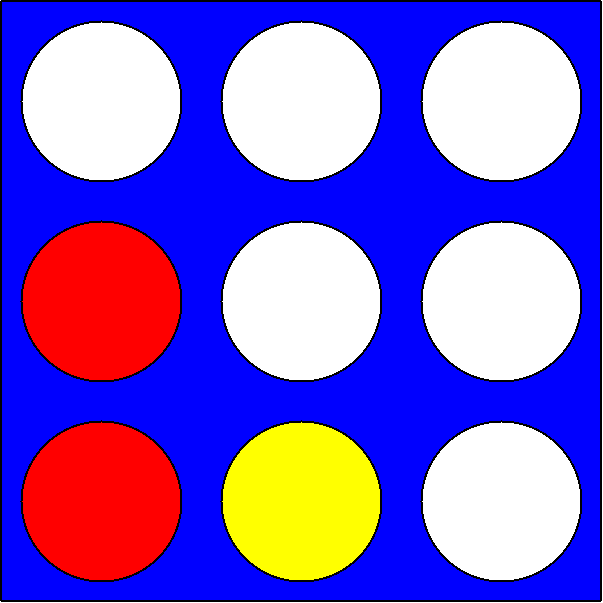
\includegraphics[width=0.25\linewidth]{images/3e.png}}%
    \only<5>{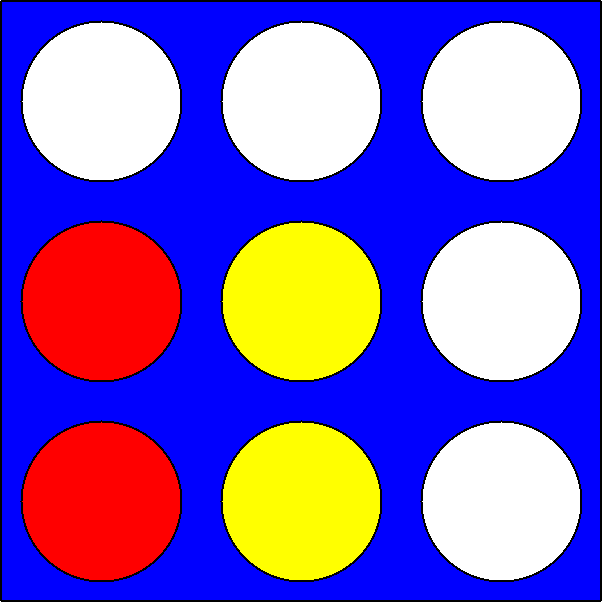
\includegraphics[width=0.25\linewidth]{images/4e.png}}%
    \only<6>{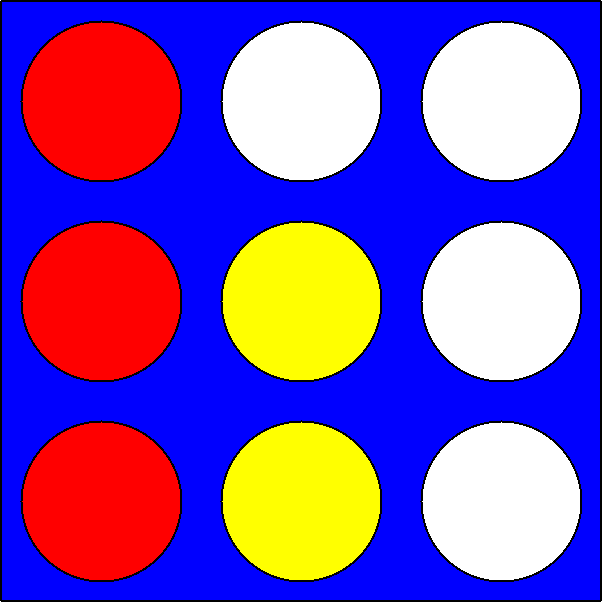
\includegraphics[width=0.25\linewidth]{images/5e.png}}%
    \only<7>{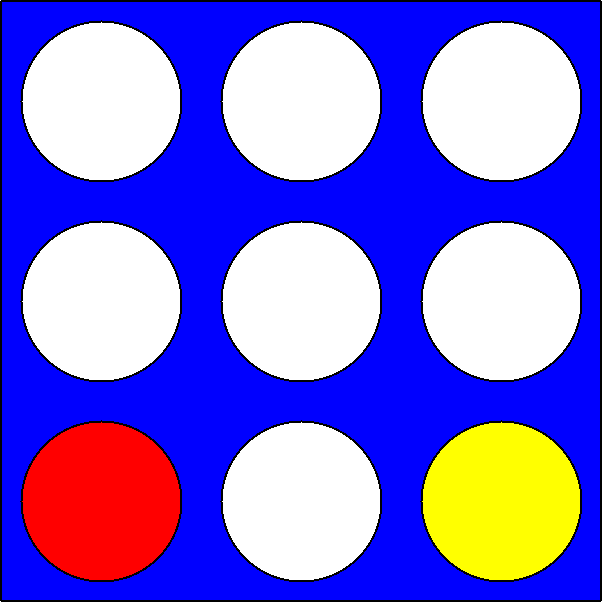
\includegraphics[width=0.25\linewidth]{images/deu.png}}%
    \only<8>{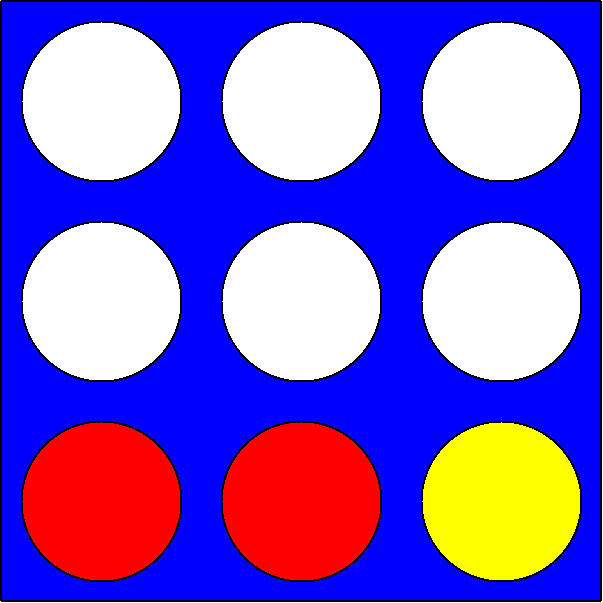
\includegraphics[width=0.25\linewidth]{images/tr.png}}%
    \only<9>{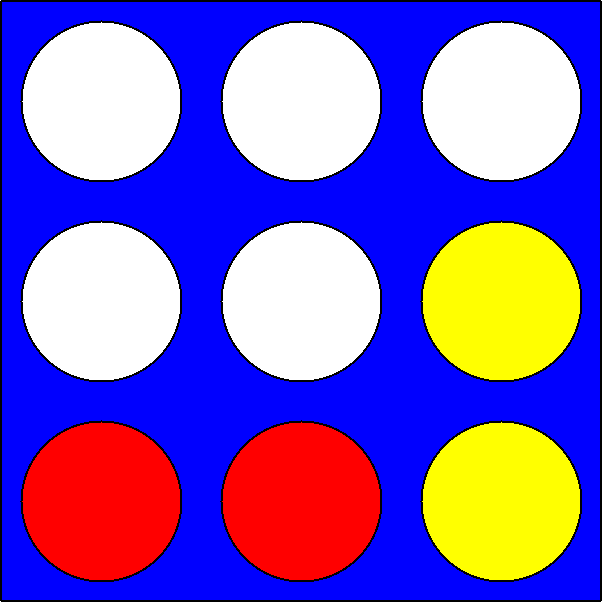
\includegraphics[width=0.25\linewidth]{images/qu.png}}%
    \only<10>{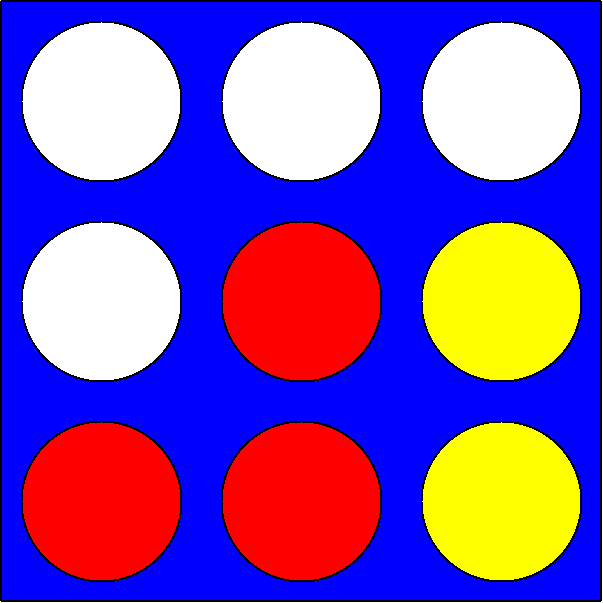
\includegraphics[width=0.25\linewidth]{images/cq.png}}%
    \only<11>{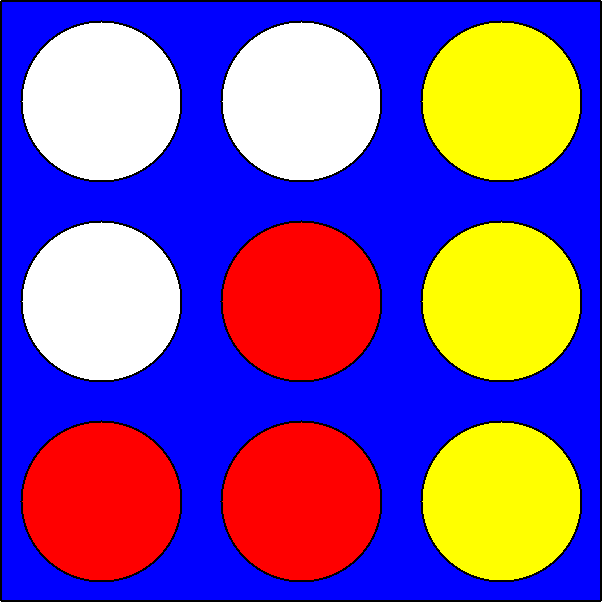
\includegraphics[width=0.25\linewidth]{images/six.png}}%
    \only<12>{%
      \rlap{\raisebox{0.3\linewidth}{%
          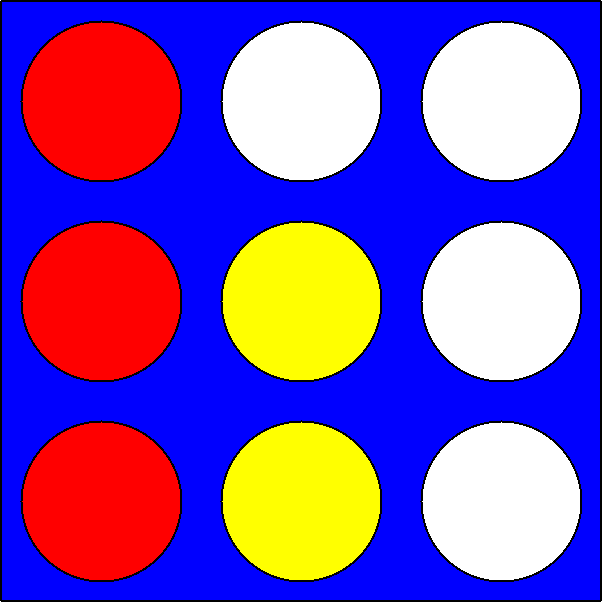
\includegraphics[width=0.25\linewidth]{images/5e.png}}}%
      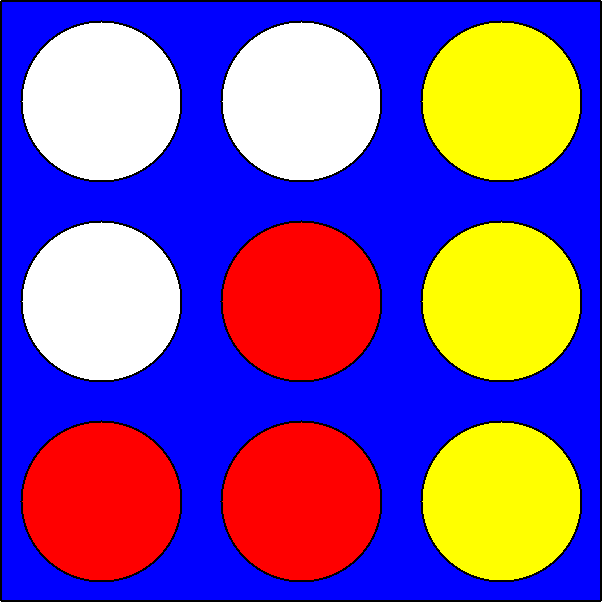
\includegraphics[width=0.25\linewidth]{images/six.png}}%

\end{frame}


\begin{frame}
\frametitle{Arbre}
	\begin{tikzpicture}[x=3em,y=2.3em,thick]
	\begin{scope}[text height=7pt]
	% Level 0-1
	\node (top) [circle,draw] at (0,0) {};
	\node (l) [circle,draw] at (-2,-1) {};
	\node (c) [circle,draw] at (0,-1) {};
	\node (r) [circle,draw] at (2,-1) {};
	\draw[->] (top) -- (l) node[above,pos=0.5]{};
	\draw[->] (top) -- (c) node[above,pos=0.5] {};
	\draw[->] (top) -- (r) node[above,pos=0.5] {};
	\end{scope}
	\begin{scope}[text height=4pt]
	% Level 1-2
	\node (ll) [circle,draw] at (-3.5,-2) {};
	\node (lc) [circle,draw] at (-2,-2) {};
	\node (lr) [circle,draw] at (-0.5,-2) {};
	\draw[->] (l) -- (ll) node[above,pos=0.5]{};
	\draw[->] (l) -- (lc) node[above,pos=0.5] {};
	\draw[->] (l) -- (lr) node[above,pos=0.5] {};
	% Level 2-3
	\node (lll) [circle,draw] at (-6,-3) {};
	\node (llc) [circle,draw] at (-3.5,-3) {};
	\node (llr) [circle,draw] at (-1,-3) {};
	\draw[->] (ll) -- (lll) node[above,pos=0.5]{};
	\draw[->] (ll) -- (llc) node[above,pos=0.5] {};
	\draw[->] (ll) -- (llr) node[above,pos=0.5] {};
	% Level 3-4
	\node (lllc) [circle,draw] at (-6,-4) {};
	\node (lllr) [circle,draw] at (-3.5,-4) {};
	\draw[->] (lll) -- (lllc) node[above,pos=0.5] {};
	\draw[->] (lll) -- (lllr) node[above,pos=0.5] {};
	\end{scope}

	\begin{scope}[text height=2pt]
	% Level 4-5
	\node (lllcc) [circle,draw] at (-6,-5) {};
	\node (lllcr) [circle,draw] at (-4.75,-5) {};
	\draw[->] (lllc) -- (lllcc) node[above,pos=0.5] {};
	\draw[->] (lllc) -- (lllcr) node[above,pos=0.5] {};
	
	\node (lllrc) [circle,draw] at (-3.5,-5) {};
	\node (lllrr) [circle,draw] at (-2.25,-5) {};
	\draw[->] (lllr) -- (lllrc) node[above,pos=0.5] {};
	\draw[->] (lllr) -- (lllrr) node[above,pos=0.5] {};
	\end{scope}

	\begin{scope}[text height=1pt]
	\node (lllccc) [circle,draw] at (-6,-6) {};
	\node (lllccr) [circle,draw] at (-5.25,-6) {};
	\draw[->] (lllcc) -- (lllccc) node[above,pos=0.5] {};
	\draw[->] (lllcc) -- (lllccr) node[above,pos=0.5] {};

	\node (lllcrc) [circle,draw] at (-4.75,-6) {};
	\node (lllcrr) [circle,draw] at (-4,-6) {};
	\draw[->] (lllcr) -- (lllcrc) node[above,pos=0.5] {};
	\draw[->] (lllcr) -- (lllcrr) node[above,pos=0.5] {};

	\node (lllrcc) [circle,draw] at (-3.5,-6) {};
	\node (lllrcr) [circle,draw] at (-2.75,-6) {};
	\draw[->] (lllrc) -- (lllrcc) node[above,pos=0.5] {};
	\draw[->] (lllrc) -- (lllrcr) node[above,pos=0.5] {};

	\node (lllrrc) [circle,draw] at (-2.25,-6) {};
	\node (lllrrr) [circle,draw] at (-1.5,-6) {};
	\draw[->] (lllrr) -- (lllrrc) node[above,pos=0.5] {};
	\draw[->] (lllrr) -- (lllrrr) node[above,pos=0.5] {};

	\node (lllcccr) [circle,draw] at (-5.8,-7) {};
	\draw[->] (lllccc) -- (lllcccr) node[above,pos=0.5] {};
	%\node (lllcccrr) [circle,draw] at (-5.7,-8) {};
	%\draw[->] (lllcccr) -- (lllcccrr) node[above,pos=0.5] {};

	\node (lllccrc) [circle,draw] at (-5.25,-7) {};
	\draw[->] (lllccr) -- (lllccrc) node[above,pos=0.5] {};
	\node (lllccrr) [circle,draw] at (-4.6,-7) {};
	\draw[->] (lllccr) -- (lllccrr) node[above,pos=0.5] {};

	\node (lllccrcr) [circle,draw] at (-5,-8) {};
	\draw[->] (lllccrc) -- (lllccrcr) node[above,pos=0.5] {};

	\node (lllccrrc) [circle,draw] at (-4.6,-8) {};
	\draw[->] (lllccrr) -- (lllccrrc) node[above,pos=0.5] {};

	\end{scope}
    \end{tikzpicture}
\end{frame}

\subsection{Généralisation}
%\frame{
%	\frametitle{Généralisation}
%	\begin{center}
%	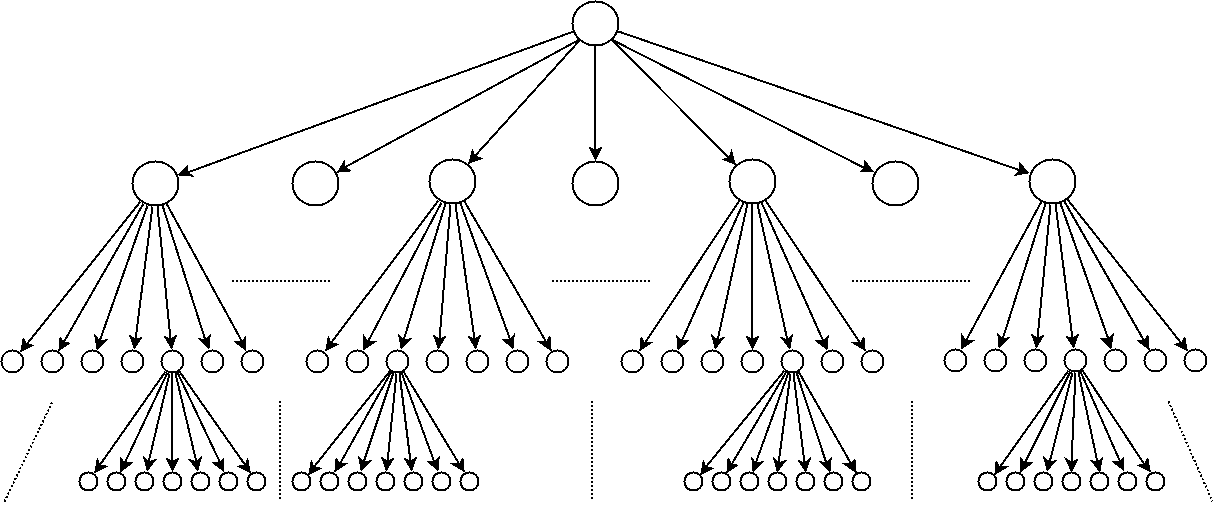
\includegraphics[width=1.\linewidth]{images/arbrePui4.png}
%	\end{center}
%}

\frame{
	\frametitle{Généralisation}
	\begin{center}
	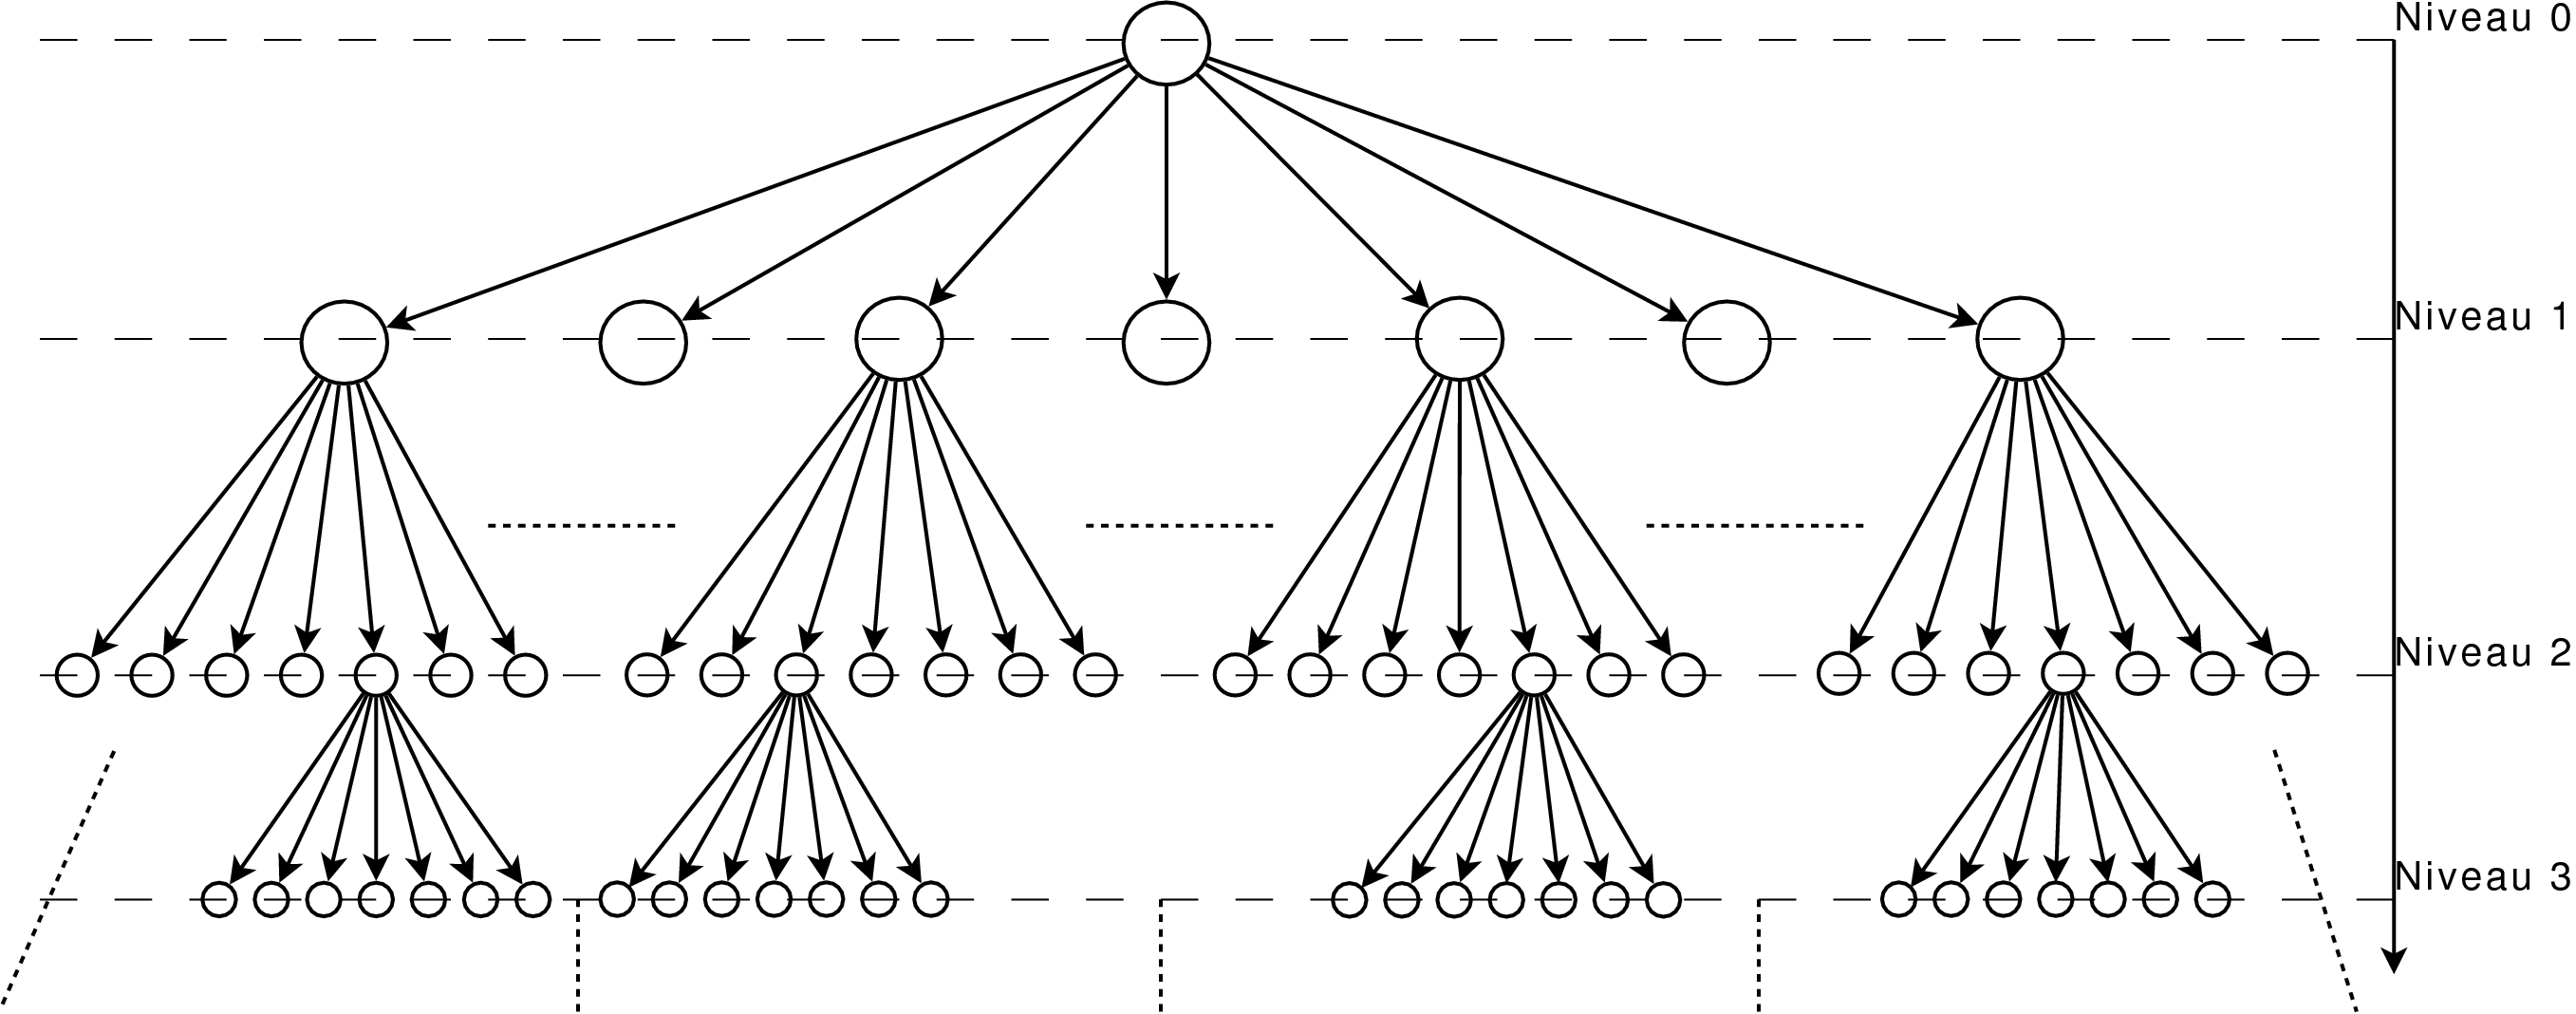
\includegraphics[width=1.\linewidth]{images/arbre7niveaux.png}
	\end{center}
}

\frame{
	\begin{table}[h]
	\begin{tabular}{c|l}
	Niveau & \ Nombre de configurations \\
	\hline
	1 & $7^{1} = 7$ \\
	2 & $7^{2} = 49$ \\
	3 & $7^{3} = 343$ \\
	4 & $7^{4} = 2.401$ \\
	5 & $7^{5} = 16.807$ \\
	6 & $7^{6} = 117.649$ \\
	7 & $7^{7} = 823.543$ \\
	8 & $7^{8} = 5.764.801$ \\
	9 & $7^{9} = 40.353.607$ \\
	10 & $7^{10} = 282.475.249$ \\
	11 & $7^{11} = 1.977.326.743$\\
	\vdots & \vdots \\
	42 & $7^{42}  \approx 3 * 10^{35}$
	\end{tabular}
	\end{table}
	\pause
	\Large{Explosion des cas!}
}
\end{document}

%\begin{frame}
%  \frametitle{Idée de l'algorithme}
%  \deroulementJeu[8em]{1er.png}{arbre1.png}{pr.png}
%\end{frame}
%
%
%\begin{frame}
%  \frametitle{Idée de l'algorithme}
%  \deroulementJeu[8em]{2e.png}{arbre2.png}{deu.png}
%\end{frame}
%
%\begin{frame}
%  \frametitle{Idée de l'algorithme}
%  \deroulementJeu[8em]{2e.png}{arbre2.png}{deu.png}
%\end{frame}
%
%\begin{frame}
%  \frametitle{Idée de l'algorithme}
%  \deroulementJeu[8em]{3e.png}{arbre3.png}{tr.png}
%\end{frame}
%
%\begin{frame}
%  \frametitle{Idée de l'algorithme}
%  \deroulementJeu[8em]{4e.png}{arbre4.png}{qu.png}
%\end{frame}
%
%\begin{frame}
%  \frametitle{Idée de l'algorithme}
%  \deroulementJeu[8em]{5e.png}{arbre5.png}{cq.png}
%\end{frame}
%
%\begin{frame}
%  \frametitle{Idée de l'algorithme}
%  \deroulementJeu[8em]{5e.png}{arbre7.png}{six.png}
%\end{frame}
%
%\subsection{Généralisation}
%\frame{
%	\frametitle{Généralisation}
%	\begin{center}
%	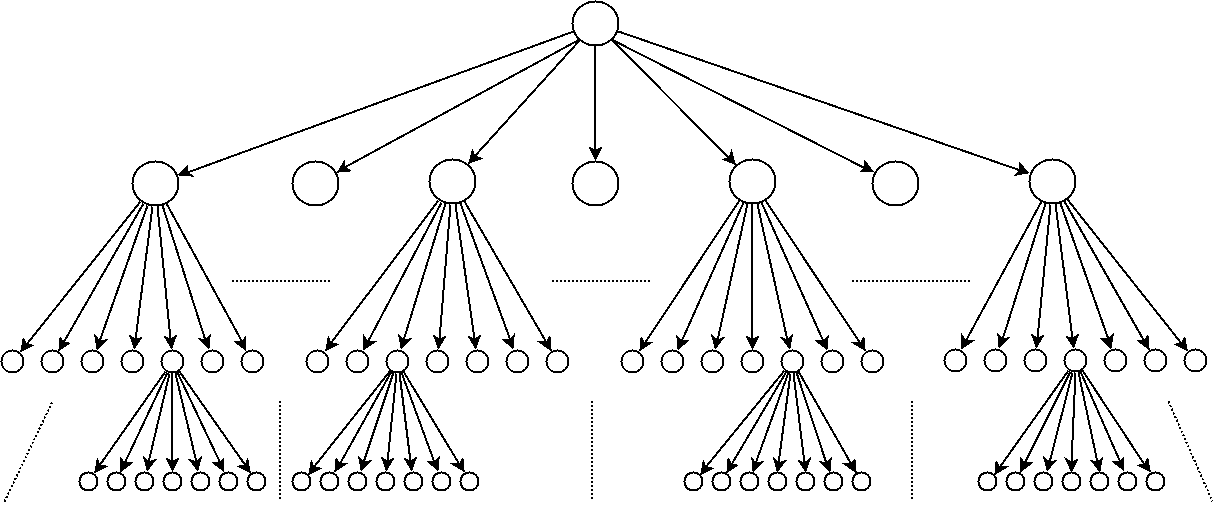
\includegraphics[width=1.\linewidth]{images/arbrePui4.png}
%	\end{center}
%}
%
%
%
%\frame{
%	\begin{table}[h]
%	\begin{tabular}{c|l}
%	Niveau & \ Nombre de configurations \\
%	\hline
%	1 & $7^{1} = 7$ \\
%	2 & $7^{2} = 49$ \\
%	3 & $7^{3} = 343$ \\
%	4 & $7^{4} = 2.401$ \\
%	5 & $7^{5} = 16.807$ \\
%	6 & $7^{6} = 117.649$ \\
%	7 & $7^{7} = 823.543$ \\
%	8 & $7^{8} = 5.764.801$ \\
%	9 & $7^{9} = 40.353.607$ \\
%	10 & $7^{10} = 282.475.249$ \\
%	11 & $7^{11} = 1.977.326.743$\\
%	\end{tabular}
%	\end{table}
%	\Large{Explosion des cas!}
%}
%
%\end{document}
